\documentclass[oneside, 11pt]{article}

\usepackage[T1]{fontenc}
\usepackage[utf8]{inputenc}
\usepackage[english]{babel}

\usepackage{fouriernc}
\usepackage[detect-all, binary-units, separate-uncertainty=true,
            per-mode=symbol, retain-explicit-plus, retain-unity-mantissa=false]{siunitx}

\usepackage{setspace}
\setstretch{1.2}

\setlength{\parskip}{\smallskipamount}
\setlength{\parindent}{0pt}

\usepackage[headheight=14pt]{geometry}
\geometry{marginparwidth=0.5cm, verbose, a4paper, tmargin=3cm, bmargin=3cm,
          lmargin=2cm, rmargin=2cm}

\usepackage{float}

\usepackage[fleqn]{amsmath}
\numberwithin{equation}{section}
\numberwithin{figure}{section}

\usepackage{graphicx}
\graphicspath{{images/}{../../../images/}}

\usepackage{tikz}
\usetikzlibrary{shapes}
\usetikzlibrary{plotmarks}

\newcounter{Exercise}
\setcounter{Exercise}{1}
\usepackage{xcolor}
\definecolor{shadecolor}{gray}{0.9}
\usepackage{framed}
\usepackage{caption}

\usepackage{url}


\usepackage{fancyhdr}
\pagestyle{fancy}
\fancyhf{}
\rhead{\thepage}
\renewcommand{\footrulewidth}{0pt}
\renewcommand{\headrulewidth}{0pt}

\fancypagestyle{firststyle}
{
    \fancyhf{}
    \rhead{\thepage}
    \cfoot{
\includegraphics[height=30pt]{HiSPARClogo}}
    \rfoot{
\includegraphics[height=25pt]{CCbysa}}
    \lfoot{
\includegraphics[height=30pt]{NIKHEFlogo}}
    \renewcommand{\footskip}{50pt}
    \renewcommand{\footrulewidth}{0.1pt}
    \renewcommand{\headrulewidth}{0pt}
}

\newcommand{\figref}[1]{Figuur~\ref{#1}}

\newcommand{\hisparc}{\textsmaller{HiSPARC}\xspace}
\newcommand{\kascade}{\textsmaller{KASCADE}\xspace}
\newcommand{\sapphire}{\textsmaller{SAPPHiRE}\xspace}
\newcommand{\jsparc}{\textsmaller{jSparc}\xspace}
\newcommand{\hdf}{\textsmaller{HDF5}\xspace}
\newcommand{\aires}{\textsmaller{AIRES}\xspace}
\newcommand{\csv}{\textsmaller{CSV}\xspace}
\newcommand{\python}{\textsmaller{PYTHON}\xspace}
\newcommand{\corsika}{\textsmaller{CORSIKA}\xspace}
\newcommand{\labview}{\textsmaller{LabVIEW}\xspace}
\newcommand{\daq}{\textsmaller{DAQ}\xspace}
\newcommand{\adc}{\textsmaller{ADC}\xspace}
\newcommand{\hi}{\textsc{h i}\xspace}
\newcommand{\hii}{\textsc{h ii}\xspace}
\newcommand{\mip}{\textsmaller{MIP}\xspace}
\newcommand{\hisparcii}{\textsmaller{HiSPARC II}\xspace}
\newcommand{\hisparciii}{\textsmaller{HiSPARC III}\xspace}

\DeclareSIUnit{\electronvolt}{\ensuremath{\mathrm{e\!\!\:V}}}

\DeclareSIUnit{\unitsigma}{\ensuremath{\sigma}}
\DeclareSIUnit{\mip}{\textsmaller{MIP}}
\DeclareSIUnit{\adc}{\textsmaller{ADC}}

\DeclareSIUnit{\gauss}{G}
\DeclareSIUnit{\parsec}{pc}
\DeclareSIUnit{\year}{yr}





%document details
\author{N.G. Schultheiss \\ translated and adapted by K. Schadenberg}
\date{}
\title{Collisions inside Air Showers}


\begin{document}
\maketitle

\section{Introduction}
In previous modules we discussed the standard model and the creation of an air shower. We briefly mentioned the energies of the individual particles and how they are formed. In this module we will take a closer look at this subject.

\section{Wavelengths}
\textbf{What is colliding with what?}

A cosmic ray hits a particle high up in the atmosphere. Lets suppose the cosmic ray was a high energy photon. Light as you might know is both a wave and a particle, or more precise it shows wave-like properties or particle-like properties depending on the situation. How can a wave collide with a particle? As a rule of thumb we can say that this only happens if the wavelength is shorter than the diameter of the particle. If the wavelength is longer it `flows' around the particle as though is was not there.

We can calculate the wavelength of a photon using the equations derived by Max Planck:
\begin{equation}
E=h \nu = h \frac{c}{\lambda}
\end{equation}
But other particles can also be seen as waves, we showed this in the module `de Broglie' for electrons. We can use the de Broglie equations to calculate the wavelength of these `particle-waves':
\begin{equation}
\lambda = \frac{h}{p} \label{eq:broglie}
\end{equation}

\begin{shaded}
\textbf{Exercise \theExercise \stepcounter{Exercise}} : Calculate the wavelength of a 0.4~kg football moving at 15.0~m/s. Compare this to the wavelength of visible light and a hydrogen-atom travelling at the speed of light. With which can you make the most accurate measurements?\end{shaded}

\begin{shaded}
\textbf{Exercise \theExercise \stepcounter{Exercise}} : The previous exercise showed that a football has a certain wavelength when it moves. However, we never see its wavelike properties, why is this?

\emph{What is the diameter of a football, how does it compare to the wavelength?} \end{shaded}

Equation~\ref{eq:broglie} shows how to use the momentum of a particle to calculate its wavelength. It is important to remember that momentum is a relativistically correct quantity. At high speeds, nearing the speed of light, one cannot simply use the product of mass and speed to calculate the momentum. We need to use a slightly modified version\footnote{See the modules `Relativity' and `de Broglie' for more details.}:
\begin{equation}
p = \gamma m_0 v \\
\end{equation}
with $m_0$ the rest mass of the particle and $\gamma$ the Lorentz factor:
\begin{equation}
\gamma = \frac{1}{\sqrt{1-\frac{v^2}{c^2}}}
\end{equation}
Equation~\ref{eq:broglie} now becomes:
\begin{equation}
\lambda = \frac{h}{m_0 v} \sqrt{1-\frac{v^2}{c^2}} \label{eq:broglie_rel}
\end{equation}

Cosmic rays can have energies in the range of GeVs, TeVs, or even higher in magnitude. In these situations we can use a short cut to calculate the de Broglie wavelength. At these energies the kinetic energy of the particle is much larger than the rest mass, allowing us to neglect the rest mass (introducing errors smaller than 1\%):
\begin{equation}
\lambda = \frac{hc}{pc}
\end{equation}
were $hc = 1239.84$~eV$\cdot$nm and $pc$ is the energy of the particle in eV.

\begin{shaded}
\textbf{Exercise \theExercise \stepcounter{Exercise}} : In the Large Hadron Collider (LHC) protons with energies up to 7~TeV are produced. Compare the wavelength of these protons with the diameter of protons and quarks at rest. Can the LHC `see' inside a proton or quark?\end{shaded}

\section{Energies}
When we want to validate a hypothesis it is convenient that we can test something under strict conditions which are always the same. Unfortunately we cannot control cosmic radiation. It question now becomes if we are able to create similar conditions in a laboratory. The most powerful particle accelerator we have at the moment is the LHC. Protons are accelerated up to energies of 7~TeV. What is the speed of the protons at this energy?
\begin{equation}
E=\gamma m c^2
\end{equation}
in which $\gamma$ is again the Lorentz factor.%\footnote{Care must be taken with these equations. Here we use $m$ to denote the relativistic mass, if we were referring to the rest mass we would have used $m_0$.}
Using the rest mass of a proton, 938.3~$\frac{\mbox{MeV}}{c^2}$:
\begin{align}
7~\mbox{TeV} &= \gamma \cdot 938.3~\mbox{MeV} \\
\gamma &= 7.5 \cdot 10^3 = \frac{1}{\sqrt{1-\frac{v^2}{c^2}}} \\
1 - \left( \frac{v}{c} \right)^2 &= 1.8 \cdot 10^{-8} \\
\beta = \frac{v}{c} &= \sqrt{1 - 1.8 \cdot 10^{-8}} \approx 1
\end{align}
We discussed the $\beta$ factor in the module `Relativity'. Being close to one means that we are talking about relativistic speeds. The same module showed that energy and momentum depend on the observer:
\begin{align}
p_{x'} &= \gamma \left( p_x - \beta \frac{E}{c} \right) \\
p_{y'} &= p_y \\
p_{z'} &= p_z \\
\frac{E'}{c} &= \gamma \left( \frac{E}{c} - \beta p_x \right) 
\end{align}
for a particle moving only in the x-direction. Momentum and energy or not invariant, rest mass is and therefore does not depend on the observer.

Collisions between cosmic rays and the atmosphere can be observed in different ways. Figure~\ref{fig:observers} part a shows us a coordinate system (frame) which is fixed to the Earth. The target of the collision is standing still. If the atmosphere is our laboratory we could also have said that we use the laboratory frame.

Figure~\ref{fig:observers} part b shows a frame moving with the cosmic ray and part c shows a frame which is fixed to the centre of gravity of the two particles involved in the collision. This last frame has the advantage that the sum of momenta equals zero.

\begin{figure}\begin{center}
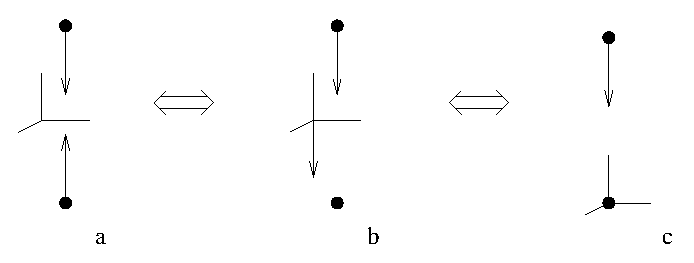
\includegraphics[scale=1]{observers}%
\caption{Coordinate systems for different observers.}\label{fig:observers}
\end{center}\end{figure}

For every observer, independent of the chosen frame, the following equation must hold:
\begin{equation}
\left(  \sum m_i^2 \right)  c^4 = \left(  \sum E_i \right)^2 + \left(  \sum p_i \right)^2 c^2 \label{eq:frame_indep}
\end{equation}

If we want to compare the energy of the moving particle colliding with a stationary particle, we can use two observers. One observer moves with the centre of gravity of the collision the other is fixed to the laboratory frame. Using the energy of the LHC, the first observer would `see':
\begin{align}
E_a = E_b &= 7~\mbox{TeV} \Rightarrow \sum E = 14~\mbox{TeV} \\
\sum p &= p_a + p_b = 0~\frac{\mbox{eV}}{c}
\end{align}
Equation~\ref{eq:frame_indep} becomes:
\begin{equation}
\left(  \sum m_i^2 \right)  c^4 = \left(  \sum E'_i \right)^2
\end{equation}
The mass is the same for both observers, this allows us to write:
\begin{equation}
\left(  \sum E'_i \right)^2 = \left(  \sum E_i \right)^2 + \left(  \sum p_i \right)^2 c^2
\end{equation}
We take the second particle (b) to be a proton:
\begin{align}
E_b &= 938.3~\mbox{MeV} \\
p_b &= 0~\frac{\mbox{kg} \cdot \mbox{m}}{\mbox{s}}
\end{align}
Using these numbers in the earlier equation yields:
\begin{equation}
\left(  14~\mbox{TeV} \right)^2 = \left(  E_a + 938.3~\mbox{MeV} \right)^2 + p_a^2 c^2 \label{eq:coll}
\end{equation}
We are left with two unknown, but related, variables; $E_a$ and $p_a$. We can use Einstein's notation for energy and rewrite the momentum as observed mass times speed. To obtain the observed mass we must again use the Lorentz factor.
\begin{align}
E &= \gamma m c^2 \\
p &= \gamma m v
\end{align}
Using the above equations to write $p$:
\begin{equation}
p = \frac{v}{c}\frac{E}{c} = \beta \frac{E}{c}
\end{equation}
Using this in equation~\ref{eq:coll}:
\begin{equation}
\left(  14~\mbox{TeV} \right)^2 = \left(  E_a + 938.3~\mbox{MeV} \right)^2 + \left(  \beta \frac{E_a}{c} \right)^2 c^2 \label{eq:coll2}
\end{equation}
We said earlier that our factor $\beta$ was nearly one, but we now have a particle moving towards an observer placed at the centre of the frame from a positive direction: $\beta \approx -1$. Therefore:
\begin{align}
\left( 14~\mbox{TeV} \right)^2 &= \left( E_a + 938.3~\mbox{MeV} \right)^2 - \left( \frac{E_a}{c} \right)^2 c^2 \Longleftrightarrow \\
\left( 14~\mbox{TeV} \right)^2 &= E_a^2 + 2 \cdot E_a \cdot 938.3~\mbox{MeV} \left( 938.3~\mbox{MeV} \right)^2 -E^2_a \Longleftrightarrow \\
\left( 14~\mbox{TeV} \right)^2 &= 2 \cdot E_a \cdot 938.3~\mbox{MeV} \left( 938.3~\mbox{MeV} \right)^2 \Longleftrightarrow \\
E_a &= \frac{\left( 14~\mbox{TeV} \right)^2 -\left( 938.3~\mbox{MeV} \right)^2 }{2 \cdot 938.3~\mbox{MeV}} = 1.0 \cdot 10^{17}~\mbox{eV}
\end{align}
Collisions with this amount of energy are relatively rare in cosmic radiation, with a single HiSPARC director we expect to measure about one each year.

\section{After the first Collision}
If we keep analysing the collisions in the centre of gravity frame the sum of momenta will always be zero, all energy is available for the creation of new particles. The calculations in the previous section showed that we have plenty energy to create a large number of different particles, including ones that are stable (enough) to reach the surface of the Earth.

The module `Air Showers' already showed us that we mostly measure muons (probably). The muon has lifetime of $2.197 \cdot 10^{-6}$~s, its heavier brother the tauon only has a lifetime of $2.906 \cdot 10^{-13}$~s, while the lightest family member the electron is stable. Travelling at the speed of light, the muon is able to travel nearly 660~m. But because of time dilation effects this becomes a few kilometres.

Why do we mostly measure muons? Even with the time dilation effect tauons decays too rapidly to reach the surface of the Earth. Electrons are stable and could reach our detectors, but these particles are easily caught by the atoms in the air causing ionisation of the air.


\begin{shaded}
\textbf{Exercise \theExercise \stepcounter{Exercise}} : Assume muons are travelling through the atmosphere at half the speed of light. How large is the distance travelled by half of the muons?\end{shaded}
\begin{shaded}
\textbf{Exercise \theExercise \stepcounter{Exercise}} : A second group of muons travels at 99\% of the speed of light. How large is the distance covered by half of these muons?\end{shaded}
\begin{shaded}
\textbf{Exercise \theExercise \stepcounter{Exercise}} : How large would your previous answer be if the particles where tauons?\end{shaded}

\end{document}

